\documentclass[]{article}
\usepackage{lmodern}
\usepackage{amssymb,amsmath}
\usepackage{ifxetex,ifluatex}
\usepackage{fixltx2e} % provides \textsubscript
\ifnum 0\ifxetex 1\fi\ifluatex 1\fi=0 % if pdftex
  \usepackage[T1]{fontenc}
  \usepackage[utf8]{inputenc}
\else % if luatex or xelatex
  \ifxetex
    \usepackage{mathspec}
  \else
    \usepackage{fontspec}
  \fi
  \defaultfontfeatures{Ligatures=TeX,Scale=MatchLowercase}
\fi
% use upquote if available, for straight quotes in verbatim environments
\IfFileExists{upquote.sty}{\usepackage{upquote}}{}
% use microtype if available
\IfFileExists{microtype.sty}{%
\usepackage{microtype}
\UseMicrotypeSet[protrusion]{basicmath} % disable protrusion for tt fonts
}{}
\usepackage[margin=1in]{geometry}
\usepackage{hyperref}
\hypersetup{unicode=true,
            pdftitle={Simulation testing of state space models in R and JD+},
            pdfauthor={Duncan Elliott},
            pdfborder={0 0 0},
            breaklinks=true}
\urlstyle{same}  % don't use monospace font for urls
\usepackage{color}
\usepackage{fancyvrb}
\newcommand{\VerbBar}{|}
\newcommand{\VERB}{\Verb[commandchars=\\\{\}]}
\DefineVerbatimEnvironment{Highlighting}{Verbatim}{commandchars=\\\{\}}
% Add ',fontsize=\small' for more characters per line
\usepackage{framed}
\definecolor{shadecolor}{RGB}{248,248,248}
\newenvironment{Shaded}{\begin{snugshade}}{\end{snugshade}}
\newcommand{\KeywordTok}[1]{\textcolor[rgb]{0.13,0.29,0.53}{\textbf{#1}}}
\newcommand{\DataTypeTok}[1]{\textcolor[rgb]{0.13,0.29,0.53}{#1}}
\newcommand{\DecValTok}[1]{\textcolor[rgb]{0.00,0.00,0.81}{#1}}
\newcommand{\BaseNTok}[1]{\textcolor[rgb]{0.00,0.00,0.81}{#1}}
\newcommand{\FloatTok}[1]{\textcolor[rgb]{0.00,0.00,0.81}{#1}}
\newcommand{\ConstantTok}[1]{\textcolor[rgb]{0.00,0.00,0.00}{#1}}
\newcommand{\CharTok}[1]{\textcolor[rgb]{0.31,0.60,0.02}{#1}}
\newcommand{\SpecialCharTok}[1]{\textcolor[rgb]{0.00,0.00,0.00}{#1}}
\newcommand{\StringTok}[1]{\textcolor[rgb]{0.31,0.60,0.02}{#1}}
\newcommand{\VerbatimStringTok}[1]{\textcolor[rgb]{0.31,0.60,0.02}{#1}}
\newcommand{\SpecialStringTok}[1]{\textcolor[rgb]{0.31,0.60,0.02}{#1}}
\newcommand{\ImportTok}[1]{#1}
\newcommand{\CommentTok}[1]{\textcolor[rgb]{0.56,0.35,0.01}{\textit{#1}}}
\newcommand{\DocumentationTok}[1]{\textcolor[rgb]{0.56,0.35,0.01}{\textbf{\textit{#1}}}}
\newcommand{\AnnotationTok}[1]{\textcolor[rgb]{0.56,0.35,0.01}{\textbf{\textit{#1}}}}
\newcommand{\CommentVarTok}[1]{\textcolor[rgb]{0.56,0.35,0.01}{\textbf{\textit{#1}}}}
\newcommand{\OtherTok}[1]{\textcolor[rgb]{0.56,0.35,0.01}{#1}}
\newcommand{\FunctionTok}[1]{\textcolor[rgb]{0.00,0.00,0.00}{#1}}
\newcommand{\VariableTok}[1]{\textcolor[rgb]{0.00,0.00,0.00}{#1}}
\newcommand{\ControlFlowTok}[1]{\textcolor[rgb]{0.13,0.29,0.53}{\textbf{#1}}}
\newcommand{\OperatorTok}[1]{\textcolor[rgb]{0.81,0.36,0.00}{\textbf{#1}}}
\newcommand{\BuiltInTok}[1]{#1}
\newcommand{\ExtensionTok}[1]{#1}
\newcommand{\PreprocessorTok}[1]{\textcolor[rgb]{0.56,0.35,0.01}{\textit{#1}}}
\newcommand{\AttributeTok}[1]{\textcolor[rgb]{0.77,0.63,0.00}{#1}}
\newcommand{\RegionMarkerTok}[1]{#1}
\newcommand{\InformationTok}[1]{\textcolor[rgb]{0.56,0.35,0.01}{\textbf{\textit{#1}}}}
\newcommand{\WarningTok}[1]{\textcolor[rgb]{0.56,0.35,0.01}{\textbf{\textit{#1}}}}
\newcommand{\AlertTok}[1]{\textcolor[rgb]{0.94,0.16,0.16}{#1}}
\newcommand{\ErrorTok}[1]{\textcolor[rgb]{0.64,0.00,0.00}{\textbf{#1}}}
\newcommand{\NormalTok}[1]{#1}
\usepackage{graphicx,grffile}
\makeatletter
\def\maxwidth{\ifdim\Gin@nat@width>\linewidth\linewidth\else\Gin@nat@width\fi}
\def\maxheight{\ifdim\Gin@nat@height>\textheight\textheight\else\Gin@nat@height\fi}
\makeatother
% Scale images if necessary, so that they will not overflow the page
% margins by default, and it is still possible to overwrite the defaults
% using explicit options in \includegraphics[width, height, ...]{}
\setkeys{Gin}{width=\maxwidth,height=\maxheight,keepaspectratio}
\IfFileExists{parskip.sty}{%
\usepackage{parskip}
}{% else
\setlength{\parindent}{0pt}
\setlength{\parskip}{6pt plus 2pt minus 1pt}
}
\setlength{\emergencystretch}{3em}  % prevent overfull lines
\providecommand{\tightlist}{%
  \setlength{\itemsep}{0pt}\setlength{\parskip}{0pt}}
\setcounter{secnumdepth}{0}
% Redefines (sub)paragraphs to behave more like sections
\ifx\paragraph\undefined\else
\let\oldparagraph\paragraph
\renewcommand{\paragraph}[1]{\oldparagraph{#1}\mbox{}}
\fi
\ifx\subparagraph\undefined\else
\let\oldsubparagraph\subparagraph
\renewcommand{\subparagraph}[1]{\oldsubparagraph{#1}\mbox{}}
\fi

%%% Use protect on footnotes to avoid problems with footnotes in titles
\let\rmarkdownfootnote\footnote%
\def\footnote{\protect\rmarkdownfootnote}

%%% Change title format to be more compact
\usepackage{titling}

% Create subtitle command for use in maketitle
\newcommand{\subtitle}[1]{
  \posttitle{
    \begin{center}\large#1\end{center}
    }
}

\setlength{\droptitle}{-2em}

  \title{Simulation testing of state space models in R and JD+}
    \pretitle{\vspace{\droptitle}\centering\huge}
  \posttitle{\par}
    \author{Duncan Elliott}
    \preauthor{\centering\large\emph}
  \postauthor{\par}
      \predate{\centering\large\emph}
  \postdate{\par}
    \date{12 March 2019}


\begin{document}
\maketitle

\section{Summary}\label{summary}

\section{What's been done}\label{whats-been-done}

\section{Simulation}\label{simulation}

\begin{Shaded}
\begin{Highlighting}[]
\KeywordTok{library}\NormalTok{(KFAS)}
\end{Highlighting}
\end{Shaded}

\begin{verbatim}
## Warning: package 'KFAS' was built under R version 3.5.2
\end{verbatim}

\begin{Shaded}
\begin{Highlighting}[]
\KeywordTok{library}\NormalTok{(rjdssf)}

\NormalTok{jd_bsm<-}\ControlFlowTok{function}\NormalTok{(x, }\DataTypeTok{nar=}\DecValTok{0}\NormalTok{)\{}
  \CommentTok{# create the model}
\NormalTok{  bsm<-}\KeywordTok{jd3_ssf_model}\NormalTok{()}
  \CommentTok{# create the components and add them to the model}
  \KeywordTok{ssf.add}\NormalTok{(bsm, }\KeywordTok{jd3_ssf_locallineartrend}\NormalTok{(}\StringTok{"ll"}\NormalTok{))}
  \KeywordTok{ssf.add}\NormalTok{(bsm, }\KeywordTok{jd3_ssf_seasonal}\NormalTok{(}\StringTok{"s"}\NormalTok{, }\DecValTok{12}\NormalTok{, }\DataTypeTok{type=}\StringTok{"Dummy"}\NormalTok{))}
  \ControlFlowTok{if}\NormalTok{ (nar }\OperatorTok{==}\StringTok{ }\DecValTok{1}\NormalTok{)\{}
    \KeywordTok{ssf.add}\NormalTok{(bsm, }\KeywordTok{jd3_ssf_sae}\NormalTok{(}\StringTok{"n"}\NormalTok{, .}\DecValTok{5}\NormalTok{, }\DataTypeTok{lag=}\DecValTok{3}\NormalTok{))}
\NormalTok{  \}}\ControlFlowTok{else} \ControlFlowTok{if}\NormalTok{ (nar }\OperatorTok{==}\StringTok{ }\DecValTok{2}\NormalTok{)\{}
    \KeywordTok{ssf.add}\NormalTok{(bsm, }\KeywordTok{jd3_ssf_sae}\NormalTok{(}\StringTok{"n"}\NormalTok{, }\KeywordTok{c}\NormalTok{(.}\DecValTok{3}\NormalTok{, .}\DecValTok{2}\NormalTok{), }\DataTypeTok{lag=}\DecValTok{3}\NormalTok{))}
\NormalTok{  \}}
  \CommentTok{# create the equation }
  \ControlFlowTok{if}\NormalTok{ (nar }\OperatorTok{==}\StringTok{ }\DecValTok{0}\NormalTok{)\{}
\NormalTok{    eq<-}\KeywordTok{jd3_ssf_equation}\NormalTok{(}\StringTok{"eq"}\NormalTok{, .}\DecValTok{01}\NormalTok{, F)}
\NormalTok{  \}}\ControlFlowTok{else}\NormalTok{\{}
\NormalTok{    eq<-}\KeywordTok{jd3_ssf_equation}\NormalTok{(}\StringTok{"eq"}\NormalTok{)}
\NormalTok{  \}}
  \KeywordTok{ssf.add}\NormalTok{(eq, }\StringTok{"ll"}\NormalTok{)}
  \KeywordTok{ssf.add}\NormalTok{(eq, }\StringTok{"s"}\NormalTok{)}
  \ControlFlowTok{if}\NormalTok{ (nar }\OperatorTok{>}\DecValTok{0}\NormalTok{)\{}
    \KeywordTok{ssf.add}\NormalTok{(eq, }\StringTok{"n"}\NormalTok{)}
\NormalTok{  \}}
  \KeywordTok{ssf.add}\NormalTok{(bsm, eq)}
  \CommentTok{#estimate the model}
\NormalTok{  rslt<-}\KeywordTok{ssf.estimate}\NormalTok{(bsm, x, }\DataTypeTok{precision=}\FloatTok{1e-9}\NormalTok{)}
\NormalTok{\}}

\NormalTok{kfas_bsm <-}\StringTok{ }\ControlFlowTok{function}\NormalTok{(x,init_val,}\DataTypeTok{optim_method=}\StringTok{"BFGS"}\NormalTok{)\{}
\NormalTok{  mdl <-}\StringTok{ }\KeywordTok{SSModel}\NormalTok{(x }\OperatorTok{~}\StringTok{ }\OperatorTok{-}\DecValTok{1}\OperatorTok{+}\KeywordTok{SSMtrend}\NormalTok{(}\DecValTok{2}\NormalTok{, }\DataTypeTok{Q =} \KeywordTok{list}\NormalTok{(}\OtherTok{NA}\NormalTok{,}\OtherTok{NA}\NormalTok{))}\OperatorTok{+}
\StringTok{   }\KeywordTok{SSMseasonal}\NormalTok{(}\DataTypeTok{period =} \DecValTok{12}\NormalTok{, }\DataTypeTok{sea.type=}\StringTok{"dummy"}\NormalTok{, }\DataTypeTok{Q =} \OtherTok{NA}\NormalTok{), }\DataTypeTok{H =} \OtherTok{NA}\NormalTok{)}
\NormalTok{  est_mdl <-}\StringTok{ }\KeywordTok{fitSSM}\NormalTok{(mdl, }\KeywordTok{rep}\NormalTok{(init_val,}\DecValTok{4}\NormalTok{),}
                  \DataTypeTok{method =}\NormalTok{ optim_method)}
\NormalTok{  mdl <-}\StringTok{ }\NormalTok{est_mdl}\OperatorTok{$}\NormalTok{model}
\NormalTok{  out <-}\StringTok{ }\KeywordTok{KFS}\NormalTok{(mdl, }\DataTypeTok{filtering =} \KeywordTok{c}\NormalTok{(}\StringTok{"state"}\NormalTok{,}\StringTok{"disturbance"}\NormalTok{), }\DataTypeTok{smoothing =} \KeywordTok{c}\NormalTok{(}\StringTok{"state"}\NormalTok{,}\StringTok{"disturbance"}\NormalTok{))}
\NormalTok{  rslt <-}\StringTok{ }\KeywordTok{list}\NormalTok{(}\DataTypeTok{hyper_est=}\NormalTok{est_mdl,}\DataTypeTok{out=}\NormalTok{out)}
  \KeywordTok{return}\NormalTok{(rslt)}
\NormalTok{\}}

\KeywordTok{set.seed}\NormalTok{(}\DecValTok{20}\NormalTok{)}

\NormalTok{y <-}\StringTok{ }\KeywordTok{rep}\NormalTok{(}\OtherTok{NA}\NormalTok{,}\DecValTok{120}\NormalTok{)}
  
\NormalTok{var_level <-}\StringTok{ }\FloatTok{0.1}
\NormalTok{var_slope <-}\StringTok{ }\FloatTok{0.3}
\NormalTok{var_seas <-}\StringTok{ }\FloatTok{0.5}
\NormalTok{var_noise <-}\StringTok{ }\FloatTok{0.7}
\NormalTok{  mdl_raw <-}\StringTok{ }\KeywordTok{SSModel}\NormalTok{(y }\OperatorTok{~}\StringTok{ }\OperatorTok{-}\DecValTok{1}\OperatorTok{+}\KeywordTok{SSMtrend}\NormalTok{(}\DecValTok{2}\NormalTok{, }\DataTypeTok{Q =} \KeywordTok{list}\NormalTok{(var_level,var_slope))}\OperatorTok{+}
\StringTok{   }\KeywordTok{SSMseasonal}\NormalTok{(}\DataTypeTok{period =} \DecValTok{12}\NormalTok{, }\DataTypeTok{sea.type=}\StringTok{"dummy"}\NormalTok{, }\DataTypeTok{Q =}\NormalTok{ var_seas), }\DataTypeTok{H =}\NormalTok{ var_noise)}
\NormalTok{init_val <-}\StringTok{ }\DecValTok{0}
\NormalTok{sim <-}\StringTok{  }\KeywordTok{simulateSSM}\NormalTok{(mdl_raw,}\DataTypeTok{type=}\StringTok{"observations"}\NormalTok{)}

\KeywordTok{ts.plot}\NormalTok{(sim)}
\end{Highlighting}
\end{Shaded}

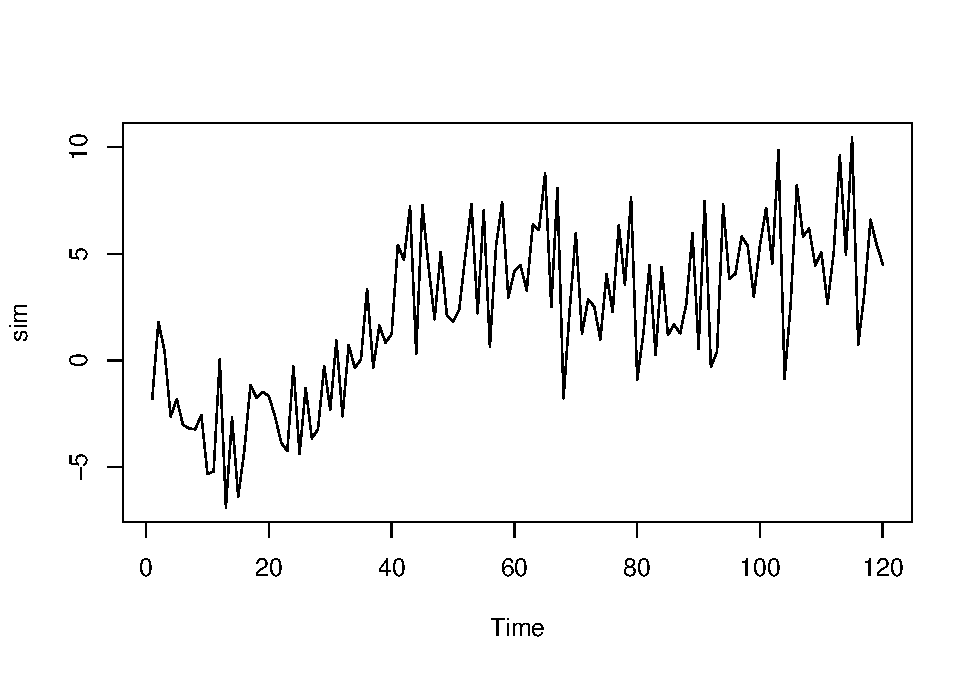
\includegraphics{simulation_test_files/figure-latex/simulate-1.pdf}

\begin{Shaded}
\begin{Highlighting}[]
\NormalTok{bsm_simul<-}\OtherTok{NULL}
\NormalTok{n <-}\StringTok{ }\DecValTok{200}
\NormalTok{sim_start <-}\StringTok{ }\KeywordTok{Sys.time}\NormalTok{()}
\NormalTok{jd_estimate <-}\StringTok{ }\OtherTok{NULL}
\NormalTok{kfas_estimate <-}\StringTok{ }\OtherTok{NULL}
\ControlFlowTok{for}\NormalTok{(i }\ControlFlowTok{in} \DecValTok{1}\OperatorTok{:}\NormalTok{n)\{}
\NormalTok{   sim <-}\StringTok{  }\KeywordTok{simulateSSM}\NormalTok{(mdl_raw,}\DataTypeTok{type=}\StringTok{"observations"}\NormalTok{)[,}\DecValTok{1}\NormalTok{,}\DecValTok{1}\NormalTok{]}
\NormalTok{   bsm_simul<-}\KeywordTok{cbind}\NormalTok{(bsm_simul, }\KeywordTok{matrix}\NormalTok{(sim, }\DecValTok{120}\NormalTok{, }\DecValTok{1}\NormalTok{))}
\NormalTok{   jd_start <-}\StringTok{ }\KeywordTok{Sys.time}\NormalTok{()}
\NormalTok{   q <-}\StringTok{ }\KeywordTok{jd_bsm}\NormalTok{(sim,}\DataTypeTok{nar=}\DecValTok{0}\NormalTok{)}
\NormalTok{   jd_end <-}\StringTok{ }\KeywordTok{Sys.time}\NormalTok{()}
\NormalTok{   jd_dur <-}\StringTok{ }\NormalTok{jd_end}\OperatorTok{-}\NormalTok{jd_start}
\NormalTok{   s <-}\StringTok{ }\KeywordTok{result}\NormalTok{(q, }\StringTok{"scalingfactor"}\NormalTok{) }
\NormalTok{   p<-}\KeywordTok{result}\NormalTok{(q, }\StringTok{"parameters"}\NormalTok{)}
\NormalTok{   jd_estimate <-}\StringTok{ }\KeywordTok{rbind}\NormalTok{(jd_estimate,}\KeywordTok{as.numeric}\NormalTok{(}\KeywordTok{c}\NormalTok{(jd_dur,}\OperatorTok{-}\DecValTok{1}\OperatorTok{*}\KeywordTok{result}\NormalTok{(q,}\StringTok{"loglikelihood"}\NormalTok{),s}\OperatorTok{*}\NormalTok{p[}\KeywordTok{c}\NormalTok{(}\DecValTok{1}\OperatorTok{:}\DecValTok{3}\NormalTok{)],s}\OperatorTok{*}\NormalTok{p[}\KeywordTok{length}\NormalTok{(p)]}\OperatorTok{*}\NormalTok{p[}\KeywordTok{length}\NormalTok{(p)])))}
\NormalTok{   kfas_start <-}\StringTok{ }\KeywordTok{Sys.time}\NormalTok{()}
\NormalTok{   r <-}\StringTok{ }\KeywordTok{kfas_bsm}\NormalTok{(sim,init_val)}
\NormalTok{   kfas_end <-}\StringTok{ }\KeywordTok{Sys.time}\NormalTok{()}
\NormalTok{   kfas_dur <-}\StringTok{ }\NormalTok{kfas_end}\OperatorTok{-}\NormalTok{kfas_start}
\NormalTok{   kfas_estimate <-}\StringTok{ }\KeywordTok{rbind}\NormalTok{(kfas_estimate, }\KeywordTok{c}\NormalTok{(kfas_dur,r}\OperatorTok{$}\NormalTok{hyper_est}\OperatorTok{$}\NormalTok{optim.out}\OperatorTok{$}\NormalTok{value,}\KeywordTok{diag}\NormalTok{(r}\OperatorTok{$}\NormalTok{out}\OperatorTok{$}\NormalTok{model}\OperatorTok{$}\NormalTok{Q[,,}\DecValTok{1}\NormalTok{]),r}\OperatorTok{$}\NormalTok{out}\OperatorTok{$}\NormalTok{model}\OperatorTok{$}\NormalTok{H[,,}\DecValTok{1}\NormalTok{]))}
\NormalTok{\}}
\NormalTok{sim_end <-}\StringTok{ }\KeywordTok{Sys.time}\NormalTok{()}
\NormalTok{sim_dur <-}\StringTok{ }\NormalTok{sim_end}\OperatorTok{-}\NormalTok{sim_start}

\KeywordTok{print}\NormalTok{(}\KeywordTok{paste}\NormalTok{(}\StringTok{"Number of simulations ="}\NormalTok{,n))}
\end{Highlighting}
\end{Shaded}

\begin{verbatim}
## [1] "Number of simulations = 200"
\end{verbatim}

\begin{Shaded}
\begin{Highlighting}[]
\KeywordTok{print}\NormalTok{(}\KeywordTok{paste}\NormalTok{(}\StringTok{"JD+ average execution time ="}\NormalTok{,}\KeywordTok{sum}\NormalTok{(jd_estimate[}\DecValTok{2}\OperatorTok{:}\NormalTok{n,}\DecValTok{1}\NormalTok{])}\OperatorTok{/}\NormalTok{(n}\OperatorTok{-}\DecValTok{1}\NormalTok{)))}
\end{Highlighting}
\end{Shaded}

\begin{verbatim}
## [1] "JD+ average execution time = 0.0347155482325722"
\end{verbatim}

\begin{Shaded}
\begin{Highlighting}[]
\KeywordTok{print}\NormalTok{(}\KeywordTok{paste}\NormalTok{(}\StringTok{"KFAS average execution time ="}\NormalTok{,}\KeywordTok{sum}\NormalTok{(kfas_estimate[}\DecValTok{2}\OperatorTok{:}\NormalTok{n,}\DecValTok{1}\NormalTok{])}\OperatorTok{/}\NormalTok{(n}\OperatorTok{-}\DecValTok{1}\NormalTok{)))}
\end{Highlighting}
\end{Shaded}

\begin{verbatim}
## [1] "KFAS average execution time = 0.217441973374717"
\end{verbatim}

\begin{Shaded}
\begin{Highlighting}[]
\KeywordTok{print}\NormalTok{(}\StringTok{"JD+ likelihood - KFAS likelihood"}\NormalTok{)}
\end{Highlighting}
\end{Shaded}

\begin{verbatim}
## [1] "JD+ likelihood - KFAS likelihood"
\end{verbatim}

\begin{Shaded}
\begin{Highlighting}[]
\KeywordTok{print}\NormalTok{(}\KeywordTok{summary}\NormalTok{(kfas_estimate[,}\DecValTok{2}\NormalTok{]}\OperatorTok{-}\NormalTok{jd_estimate[,}\DecValTok{2}\NormalTok{]))}
\end{Highlighting}
\end{Shaded}

\begin{verbatim}
##       Min.    1st Qu.     Median       Mean    3rd Qu.       Max. 
## -1.810e-07  2.590e-07  5.332e-04  8.716e-04  1.481e-03  5.311e-03
\end{verbatim}

\begin{Shaded}
\begin{Highlighting}[]
\NormalTok{est_nams <-}\StringTok{ }\KeywordTok{c}\NormalTok{(}\StringTok{"Run time per series"}\NormalTok{,}\StringTok{"Negative Loglikelihood"}\NormalTok{,}\StringTok{"Level Variance"}\NormalTok{,}\StringTok{"Slope Variance"}\NormalTok{,}\StringTok{"Seasonal Variance"}\NormalTok{,}\StringTok{"Observation variance"}\NormalTok{)}
\ControlFlowTok{for}\NormalTok{(i }\ControlFlowTok{in} \DecValTok{1}\OperatorTok{:}\KeywordTok{ncol}\NormalTok{(jd_estimate))\{}
  \KeywordTok{boxplot}\NormalTok{(}\KeywordTok{data.frame}\NormalTok{(}\DataTypeTok{JD=}\NormalTok{jd_estimate[,i],}\DataTypeTok{KFAS=}\NormalTok{kfas_estimate[,i]),}\DataTypeTok{main=}\NormalTok{est_nams[i])}
  \ControlFlowTok{if}\NormalTok{(i}\OperatorTok{==}\DecValTok{3}\NormalTok{)\{}\KeywordTok{abline}\NormalTok{(}\DataTypeTok{h=}\NormalTok{var_level,}\DataTypeTok{lty=}\DecValTok{2}\NormalTok{,}\DataTypeTok{col=}\DecValTok{2}\NormalTok{)\}}
  \ControlFlowTok{if}\NormalTok{(i}\OperatorTok{==}\DecValTok{4}\NormalTok{)\{}\KeywordTok{abline}\NormalTok{(}\DataTypeTok{h=}\NormalTok{var_slope,}\DataTypeTok{lty=}\DecValTok{2}\NormalTok{,}\DataTypeTok{col=}\DecValTok{2}\NormalTok{)\}}
  \ControlFlowTok{if}\NormalTok{(i}\OperatorTok{==}\DecValTok{5}\NormalTok{)\{}\KeywordTok{abline}\NormalTok{(}\DataTypeTok{h=}\NormalTok{var_seas,}\DataTypeTok{lty=}\DecValTok{2}\NormalTok{,}\DataTypeTok{col=}\DecValTok{2}\NormalTok{)\}}
  \ControlFlowTok{if}\NormalTok{(i}\OperatorTok{==}\DecValTok{6}\NormalTok{)\{}\KeywordTok{abline}\NormalTok{(}\DataTypeTok{h=}\NormalTok{var_noise,}\DataTypeTok{lty=}\DecValTok{2}\NormalTok{,}\DataTypeTok{col=}\DecValTok{2}\NormalTok{)\}}
\NormalTok{\}}
\end{Highlighting}
\end{Shaded}

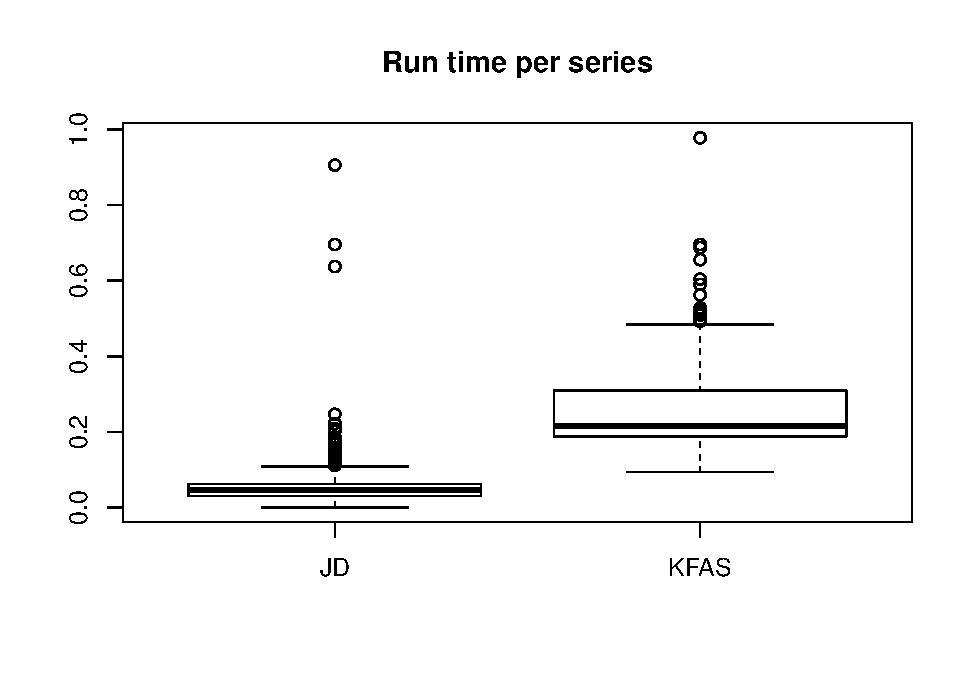
\includegraphics{simulation_test_files/figure-latex/simulate-2.pdf}
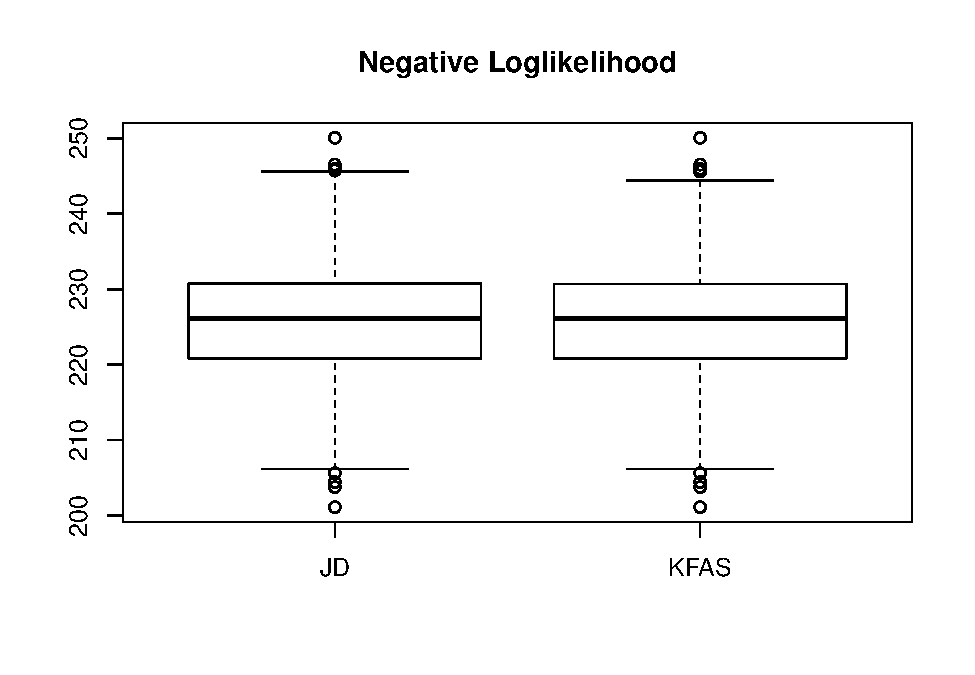
\includegraphics{simulation_test_files/figure-latex/simulate-3.pdf}
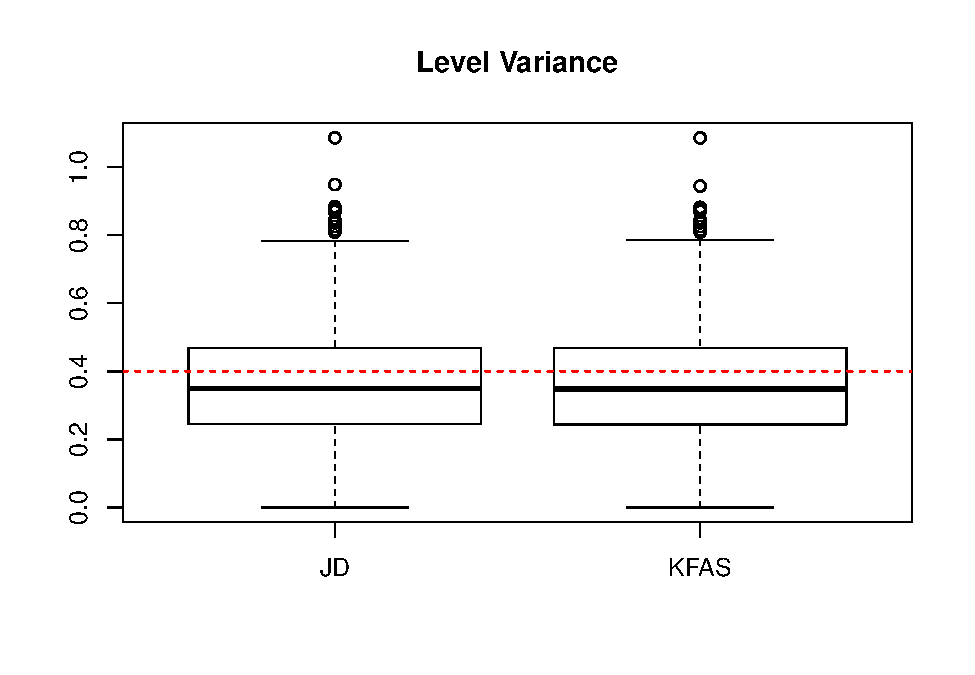
\includegraphics{simulation_test_files/figure-latex/simulate-4.pdf}
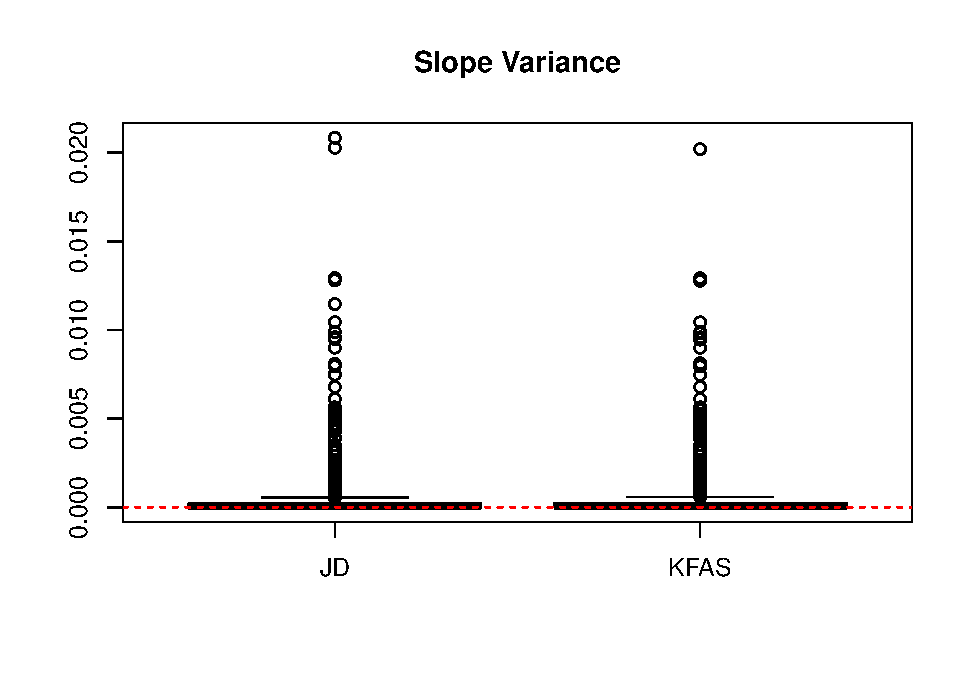
\includegraphics{simulation_test_files/figure-latex/simulate-5.pdf}
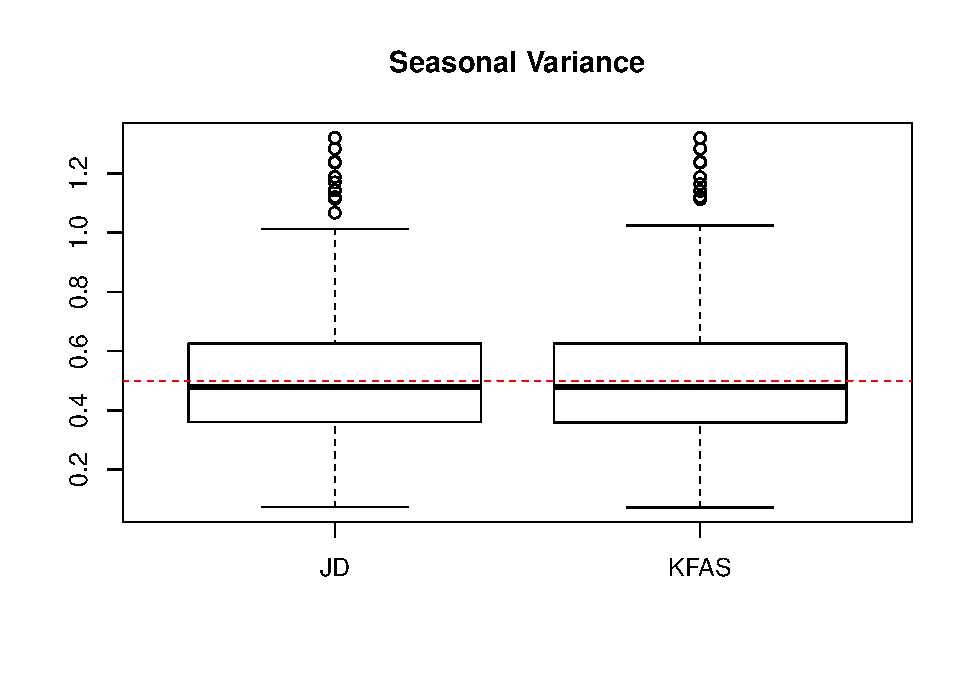
\includegraphics{simulation_test_files/figure-latex/simulate-6.pdf}
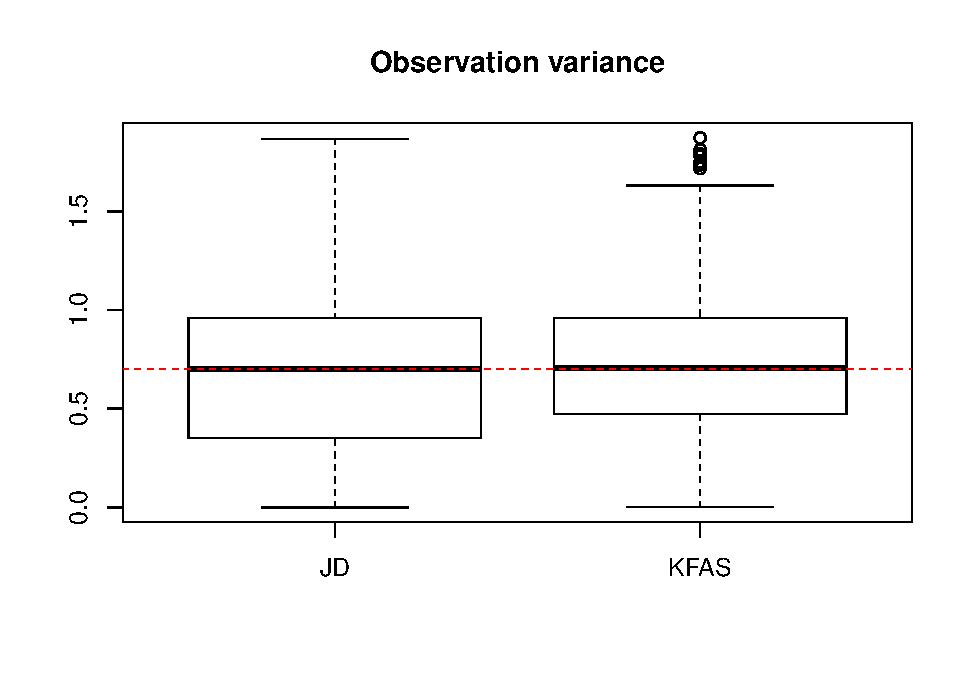
\includegraphics{simulation_test_files/figure-latex/simulate-7.pdf} \#
Simulation of sampling error autocorrelation variances only Ie assume
the correlation is known

\begin{Shaded}
\begin{Highlighting}[]
\NormalTok{  rho.}\DecValTok{1}\NormalTok{ <-}\StringTok{ }\DecValTok{0}     \CommentTok{# value of wave1  AR coefficient}
\NormalTok{  rho.}\DecValTok{2}\NormalTok{ <-}\StringTok{ }\FloatTok{0.8}                       \CommentTok{# value of wave 2  AR coefficient}
\NormalTok{  rho.}\DecValTok{3}\NormalTok{ <-}\StringTok{ }\FloatTok{0.7}                       \CommentTok{# value of wave 3 AR coefficient}
\NormalTok{  rho.}\DecValTok{4}\NormalTok{ <-}\StringTok{ }\FloatTok{0.6}                       \CommentTok{# value of wave 4 AR coefficient}
\NormalTok{  rho.}\DecValTok{5}\NormalTok{ <-}\StringTok{ }\FloatTok{0.8}                       \CommentTok{# value of second AR coefficient}
\NormalTok{  var1 <-}\StringTok{ }\DecValTok{1}
\NormalTok{  var2 <-}\StringTok{ }\DecValTok{2}
\NormalTok{  var3 <-}\StringTok{ }\DecValTok{3}
\NormalTok{  var4 <-}\StringTok{ }\DecValTok{4}
\NormalTok{  var5 <-}\StringTok{ }\DecValTok{5}

\NormalTok{  data.len<-}\DecValTok{60}    
    
\NormalTok{  obs.matrix.err <-}\StringTok{ }\KeywordTok{cbind}\NormalTok{(}\KeywordTok{diag}\NormalTok{(}\DecValTok{1}\NormalTok{,}\DecValTok{5}\NormalTok{),}\KeywordTok{matrix}\NormalTok{(}\DecValTok{0}\NormalTok{,}\DataTypeTok{nrow=}\DecValTok{5}\NormalTok{,}\DataTypeTok{ncol=}\DecValTok{8}\NormalTok{))}

\NormalTok{  trans.matrix.err <-}\StringTok{ }\KeywordTok{rbind}\NormalTok{(}\KeywordTok{matrix}\NormalTok{(}\DecValTok{0}\NormalTok{,}\DecValTok{1}\NormalTok{,}\DecValTok{13}\NormalTok{),}
          \KeywordTok{cbind}\NormalTok{(}\KeywordTok{matrix}\NormalTok{(}\DecValTok{0}\NormalTok{,}\DecValTok{4}\NormalTok{,}\DecValTok{9}\NormalTok{),}\KeywordTok{diag}\NormalTok{(}\KeywordTok{c}\NormalTok{(rho.}\DecValTok{2}\NormalTok{,rho.}\DecValTok{3}\NormalTok{,rho.}\DecValTok{4}\NormalTok{,rho.}\DecValTok{5}\NormalTok{))),}
          \KeywordTok{cbind}\NormalTok{(}\KeywordTok{diag}\NormalTok{(}\DecValTok{4}\NormalTok{),}\KeywordTok{matrix}\NormalTok{(}\DecValTok{0}\NormalTok{,}\DecValTok{4}\NormalTok{,}\DecValTok{9}\NormalTok{)),}
          \KeywordTok{cbind}\NormalTok{(}\KeywordTok{matrix}\NormalTok{(}\DecValTok{0}\NormalTok{,}\DecValTok{4}\NormalTok{,}\DecValTok{5}\NormalTok{),}\KeywordTok{diag}\NormalTok{(}\DecValTok{4}\NormalTok{),}\KeywordTok{matrix}\NormalTok{(}\DecValTok{0}\NormalTok{,}\DecValTok{4}\NormalTok{,}\DecValTok{4}\NormalTok{))}
\NormalTok{    )}
\NormalTok{Z_mat <-}\StringTok{ }\NormalTok{obs.matrix.err}
\NormalTok{T_mat <-}\StringTok{ }\NormalTok{trans.matrix.err}
\NormalTok{H_mat <-}\StringTok{ }\KeywordTok{diag}\NormalTok{(}\DecValTok{0}\NormalTok{,}\DecValTok{5}\NormalTok{)}\OperatorTok{*}\DecValTok{1}
\NormalTok{R_mat <-}\StringTok{ }\KeywordTok{matrix}\NormalTok{(}\DecValTok{0}\NormalTok{,}\DecValTok{13}\NormalTok{,}\DecValTok{5}\NormalTok{)}
\NormalTok{R_mat[}\DecValTok{1}\NormalTok{,}\DecValTok{1}\NormalTok{] <-}\StringTok{ }\DecValTok{1}  \CommentTok{#error w1 variance}
\NormalTok{R_mat[}\DecValTok{2}\NormalTok{,}\DecValTok{2}\NormalTok{] <-}\StringTok{ }\KeywordTok{sqrt}\NormalTok{(}\DecValTok{1}\OperatorTok{-}\NormalTok{rho.}\DecValTok{2}\OperatorTok{^}\DecValTok{2}\NormalTok{)  }\CommentTok{#error w2 variance}
\NormalTok{R_mat[}\DecValTok{3}\NormalTok{,}\DecValTok{3}\NormalTok{] <-}\StringTok{ }\KeywordTok{sqrt}\NormalTok{(}\DecValTok{1}\OperatorTok{-}\NormalTok{rho.}\DecValTok{3}\OperatorTok{^}\DecValTok{2}\NormalTok{)  }\CommentTok{#error w3 variance}
\NormalTok{R_mat[}\DecValTok{4}\NormalTok{,}\DecValTok{4}\NormalTok{] <-}\StringTok{ }\KeywordTok{sqrt}\NormalTok{(}\DecValTok{1}\OperatorTok{-}\NormalTok{rho.}\DecValTok{4}\OperatorTok{^}\DecValTok{2}\NormalTok{)  }\CommentTok{#error w4 variance}
\NormalTok{R_mat[}\DecValTok{5}\NormalTok{,}\DecValTok{5}\NormalTok{] <-}\StringTok{ }\KeywordTok{sqrt}\NormalTok{(}\DecValTok{1}\OperatorTok{-}\NormalTok{rho.}\DecValTok{5}\OperatorTok{^}\DecValTok{2}\NormalTok{)  }\CommentTok{#error w5 variance }

\NormalTok{Q_mat <-}\StringTok{ }\KeywordTok{diag}\NormalTok{(}\KeywordTok{c}\NormalTok{(var1,var2,var3,var4,var5))}

\NormalTok{se <-}\StringTok{ }\KeywordTok{matrix}\NormalTok{(}\OtherTok{NA}\NormalTok{,data.len,}\DecValTok{5}\NormalTok{)}

\NormalTok{mdl_raw2 <-}\StringTok{ }\KeywordTok{SSModel}\NormalTok{(se }\OperatorTok{~}\StringTok{ }\OperatorTok{-}\DecValTok{1}\OperatorTok{+}\KeywordTok{SSMcustom}\NormalTok{(Z_mat, T_mat, R_mat, }\DataTypeTok{Q =}\NormalTok{ Q_mat,}\DataTypeTok{P1=}\KeywordTok{diag}\NormalTok{(}\DecValTok{13}\NormalTok{)), }\DataTypeTok{H =}\NormalTok{ H_mat)}
\NormalTok{sim <-}\StringTok{  }\KeywordTok{simulateSSM}\NormalTok{(mdl_raw2,}\DataTypeTok{type=}\StringTok{"observations"}\NormalTok{)[,,}\DecValTok{1}\NormalTok{]}

\KeywordTok{acf}\NormalTok{(sim)}
\end{Highlighting}
\end{Shaded}

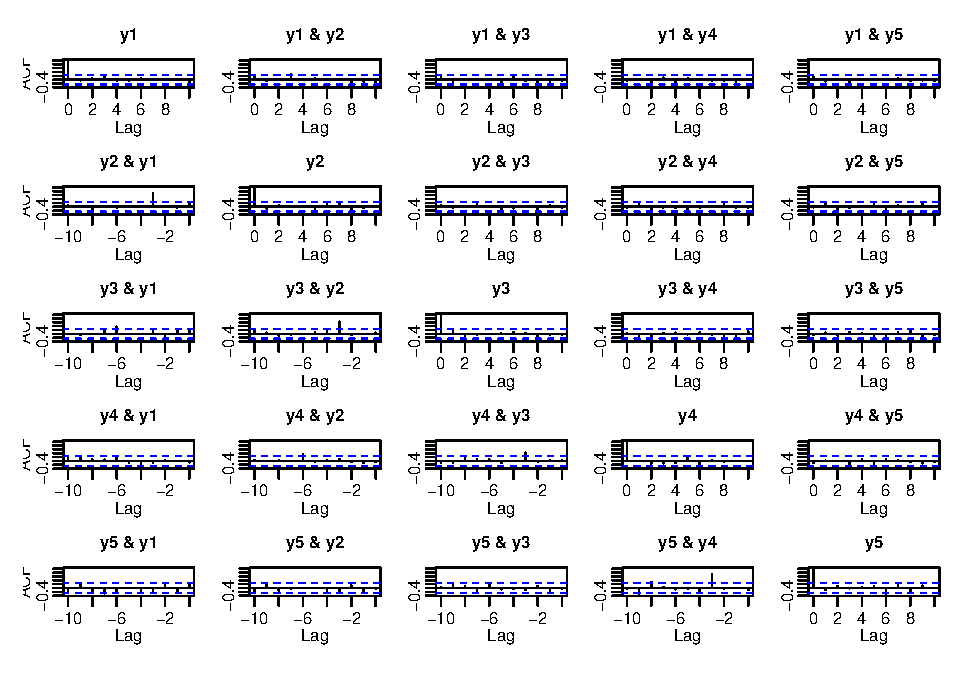
\includegraphics{simulation_test_files/figure-latex/simulate_sae-1.pdf}

\begin{Shaded}
\begin{Highlighting}[]
\NormalTok{v_tv <-}\StringTok{ }\KeywordTok{matrix}\NormalTok{(}\DecValTok{1}\NormalTok{,}\DecValTok{1}\NormalTok{,}\DecValTok{5}\NormalTok{)}

\NormalTok{jd_sae_only<-}\ControlFlowTok{function}\NormalTok{(x, }\DataTypeTok{ar=}\KeywordTok{c}\NormalTok{(rho.}\DecValTok{2}\NormalTok{,rho.}\DecValTok{3}\NormalTok{,rho.}\DecValTok{4}\NormalTok{,rho.}\DecValTok{5}\NormalTok{),}\DataTypeTok{v=}\NormalTok{v_tv)\{}
  \CommentTok{# create the model}
\NormalTok{  ons<-}\KeywordTok{jd3_ssf_model}\NormalTok{()}
  
  \CommentTok{# multivariate survey errors }
  \CommentTok{# 5 waves, ar(1) models, given r2...r5 (fixed here to .22... 25), lag = 3}
  \KeywordTok{add}\NormalTok{(ons, }\KeywordTok{jd3_ssf_msae3}\NormalTok{(}\StringTok{"sae"}\NormalTok{,}\KeywordTok{array}\NormalTok{(}\FloatTok{0.01}\NormalTok{, }\DecValTok{5}\NormalTok{), F, }\DataTypeTok{ar=}\NormalTok{ar, }\DataTypeTok{fixedar =}\NormalTok{ T, v, }\DataTypeTok{lag=}\DecValTok{3}\NormalTok{))}
  
  \CommentTok{# survey errors (set to 1.x for wave x + some noise)}
  
  \CommentTok{# create the equations }
\NormalTok{  eq1<-}\KeywordTok{jd3_ssf_equation}\NormalTok{(}\StringTok{"eq1"}\NormalTok{, }\DecValTok{0}\NormalTok{, T)}
  \KeywordTok{ssf.add}\NormalTok{(eq1, }\StringTok{"sae"}\NormalTok{, }\DataTypeTok{loading=}\KeywordTok{jd3_ssf_loading}\NormalTok{(}\DecValTok{0}\NormalTok{))}
  \KeywordTok{ssf.add}\NormalTok{(ons,eq1)}
\NormalTok{  eq2<-}\KeywordTok{jd3_ssf_equation}\NormalTok{(}\StringTok{"eq2"}\NormalTok{, }\DecValTok{0}\NormalTok{, T)}
  \KeywordTok{ssf.add}\NormalTok{(eq2, }\StringTok{"sae"}\NormalTok{, }\DataTypeTok{loading=}\KeywordTok{jd3_ssf_loading}\NormalTok{(}\DecValTok{1}\NormalTok{))}
  \KeywordTok{ssf.add}\NormalTok{(ons,eq2)}
\NormalTok{  eq3<-}\KeywordTok{jd3_ssf_equation}\NormalTok{(}\StringTok{"eq3"}\NormalTok{, }\DecValTok{0}\NormalTok{, T)}
  \KeywordTok{ssf.add}\NormalTok{(eq3, }\StringTok{"sae"}\NormalTok{, }\DataTypeTok{loading=}\KeywordTok{jd3_ssf_loading}\NormalTok{(}\DecValTok{2}\NormalTok{))}
  \KeywordTok{ssf.add}\NormalTok{(ons, eq3)}
\NormalTok{  eq4<-}\KeywordTok{jd3_ssf_equation}\NormalTok{(}\StringTok{"eq4"}\NormalTok{, }\DecValTok{0}\NormalTok{, T)}
  \KeywordTok{ssf.add}\NormalTok{(eq4, }\StringTok{"sae"}\NormalTok{, }\DataTypeTok{loading=}\KeywordTok{jd3_ssf_loading}\NormalTok{(}\DecValTok{3}\NormalTok{))}
  \KeywordTok{ssf.add}\NormalTok{(ons, eq4)}
\NormalTok{  eq5<-}\KeywordTok{jd3_ssf_equation}\NormalTok{(}\StringTok{"eq5"}\NormalTok{, }\DecValTok{0}\NormalTok{, T)}
  \KeywordTok{ssf.add}\NormalTok{(eq5, }\StringTok{"sae"}\NormalTok{, }\DataTypeTok{loading=}\KeywordTok{jd3_ssf_loading}\NormalTok{(}\DecValTok{4}\NormalTok{))}
  \KeywordTok{ssf.add}\NormalTok{(ons, eq5)}
  \KeywordTok{return}\NormalTok{ (}\KeywordTok{ssf.estimate}\NormalTok{(ons, x, }\DataTypeTok{precision=}\FloatTok{1e-9}\NormalTok{))}
\NormalTok{\}}

   
\NormalTok{kfas_sae <-}\StringTok{ }\ControlFlowTok{function}\NormalTok{(x,init_val,}\DataTypeTok{optim_method=}\StringTok{"BFGS"}\NormalTok{)\{}
\NormalTok{  obs.matrix.err <-}\StringTok{ }\KeywordTok{cbind}\NormalTok{(}\KeywordTok{diag}\NormalTok{(}\DecValTok{1}\NormalTok{,}\DecValTok{5}\NormalTok{),}\KeywordTok{matrix}\NormalTok{(}\DecValTok{0}\NormalTok{,}\DataTypeTok{nrow=}\DecValTok{5}\NormalTok{,}\DataTypeTok{ncol=}\DecValTok{8}\NormalTok{))}

\NormalTok{  trans.matrix.err <-}\StringTok{ }\KeywordTok{rbind}\NormalTok{(}\KeywordTok{matrix}\NormalTok{(}\DecValTok{0}\NormalTok{,}\DecValTok{1}\NormalTok{,}\DecValTok{13}\NormalTok{),}
          \KeywordTok{cbind}\NormalTok{(}\KeywordTok{matrix}\NormalTok{(}\DecValTok{0}\NormalTok{,}\DecValTok{4}\NormalTok{,}\DecValTok{9}\NormalTok{),}\KeywordTok{diag}\NormalTok{(}\KeywordTok{c}\NormalTok{(rho.}\DecValTok{2}\NormalTok{,rho.}\DecValTok{3}\NormalTok{,rho.}\DecValTok{4}\NormalTok{,rho.}\DecValTok{5}\NormalTok{))),}
          \KeywordTok{cbind}\NormalTok{(}\KeywordTok{diag}\NormalTok{(}\DecValTok{4}\NormalTok{),}\KeywordTok{matrix}\NormalTok{(}\DecValTok{0}\NormalTok{,}\DecValTok{4}\NormalTok{,}\DecValTok{9}\NormalTok{)),}
          \KeywordTok{cbind}\NormalTok{(}\KeywordTok{matrix}\NormalTok{(}\DecValTok{0}\NormalTok{,}\DecValTok{4}\NormalTok{,}\DecValTok{5}\NormalTok{),}\KeywordTok{diag}\NormalTok{(}\DecValTok{4}\NormalTok{),}\KeywordTok{matrix}\NormalTok{(}\DecValTok{0}\NormalTok{,}\DecValTok{4}\NormalTok{,}\DecValTok{4}\NormalTok{))}
\NormalTok{    )}
\NormalTok{   Z_mat <-}\StringTok{ }\NormalTok{obs.matrix.err}
\NormalTok{   T_mat <-}\StringTok{ }\NormalTok{trans.matrix.err}
\NormalTok{   H_mat <-}\StringTok{ }\KeywordTok{diag}\NormalTok{(}\DecValTok{0}\NormalTok{,}\DecValTok{5}\NormalTok{)}\OperatorTok{*}\DecValTok{1}
\NormalTok{   R_mat <-}\StringTok{ }\KeywordTok{matrix}\NormalTok{(}\DecValTok{0}\NormalTok{,}\DecValTok{13}\NormalTok{,}\DecValTok{5}\NormalTok{)}
\NormalTok{   R_mat[}\DecValTok{1}\NormalTok{,}\DecValTok{1}\NormalTok{] <-}\StringTok{ }\DecValTok{1}  \CommentTok{#error w1 variance}
\NormalTok{   R_mat[}\DecValTok{2}\NormalTok{,}\DecValTok{2}\NormalTok{] <-}\StringTok{ }\KeywordTok{sqrt}\NormalTok{(}\DecValTok{1}\OperatorTok{-}\NormalTok{rho.}\DecValTok{2}\OperatorTok{^}\DecValTok{2}\NormalTok{)  }\CommentTok{#error w2 variance}
\NormalTok{   R_mat[}\DecValTok{3}\NormalTok{,}\DecValTok{3}\NormalTok{] <-}\StringTok{ }\KeywordTok{sqrt}\NormalTok{(}\DecValTok{1}\OperatorTok{-}\NormalTok{rho.}\DecValTok{3}\OperatorTok{^}\DecValTok{2}\NormalTok{)  }\CommentTok{#error w3 variance}
\NormalTok{   R_mat[}\DecValTok{4}\NormalTok{,}\DecValTok{4}\NormalTok{] <-}\StringTok{ }\KeywordTok{sqrt}\NormalTok{(}\DecValTok{1}\OperatorTok{-}\NormalTok{rho.}\DecValTok{4}\OperatorTok{^}\DecValTok{2}\NormalTok{)  }\CommentTok{#error w4 variance}
\NormalTok{   R_mat[}\DecValTok{5}\NormalTok{,}\DecValTok{5}\NormalTok{] <-}\StringTok{ }\KeywordTok{sqrt}\NormalTok{(}\DecValTok{1}\OperatorTok{-}\NormalTok{rho.}\DecValTok{5}\OperatorTok{^}\DecValTok{2}\NormalTok{)  }\CommentTok{#error w5 variance }

\NormalTok{   Q_mat <-}\StringTok{ }\KeywordTok{diag}\NormalTok{(}\KeywordTok{c}\NormalTok{(}\OtherTok{NA}\NormalTok{,}\OtherTok{NA}\NormalTok{,}\OtherTok{NA}\NormalTok{,}\OtherTok{NA}\NormalTok{,}\OtherTok{NA}\NormalTok{))}

\NormalTok{   mdl <-}\StringTok{ }\KeywordTok{SSModel}\NormalTok{(x }\OperatorTok{~}\StringTok{ }\OperatorTok{-}\DecValTok{1}\OperatorTok{+}\KeywordTok{SSMcustom}\NormalTok{(Z_mat, T_mat, R_mat, }\DataTypeTok{Q =}\NormalTok{ Q_mat,}\DataTypeTok{P1=}\KeywordTok{diag}\NormalTok{(}\DecValTok{13}\NormalTok{)), }\DataTypeTok{H =}\NormalTok{ H_mat)}
\NormalTok{   est_mdl <-}\StringTok{ }\KeywordTok{fitSSM}\NormalTok{(mdl, }\KeywordTok{rep}\NormalTok{(init_val,}\DecValTok{5}\NormalTok{),}
                  \DataTypeTok{method =}\NormalTok{ optim_method)}
\NormalTok{   mdl <-}\StringTok{ }\NormalTok{est_mdl}\OperatorTok{$}\NormalTok{model}
\NormalTok{   out <-}\StringTok{ }\KeywordTok{KFS}\NormalTok{(mdl, }\DataTypeTok{filtering =} \KeywordTok{c}\NormalTok{(}\StringTok{"state"}\NormalTok{,}\StringTok{"disturbance"}\NormalTok{), }\DataTypeTok{smoothing =} \KeywordTok{c}\NormalTok{(}\StringTok{"state"}\NormalTok{,}\StringTok{"disturbance"}\NormalTok{))}
\NormalTok{   rslt <-}\StringTok{ }\KeywordTok{list}\NormalTok{(}\DataTypeTok{hyper_est=}\NormalTok{est_mdl,}\DataTypeTok{out=}\NormalTok{out)}
   \KeywordTok{return}\NormalTok{(rslt)}
\NormalTok{\}}




\NormalTok{n <-}\StringTok{ }\DecValTok{200}
\NormalTok{sim_start <-}\StringTok{ }\KeywordTok{Sys.time}\NormalTok{()}
\NormalTok{jd_estimate <-}\StringTok{ }\OtherTok{NULL}
\NormalTok{kfas_estimate <-}\StringTok{ }\OtherTok{NULL}
\ControlFlowTok{for}\NormalTok{(i }\ControlFlowTok{in} \DecValTok{1}\OperatorTok{:}\NormalTok{n)\{}
\NormalTok{   sim <-}\StringTok{  }\KeywordTok{simulateSSM}\NormalTok{(mdl_raw2,}\DataTypeTok{type=}\StringTok{"observations"}\NormalTok{)[,,}\DecValTok{1}\NormalTok{]}
\NormalTok{   jd_start <-}\StringTok{ }\KeywordTok{Sys.time}\NormalTok{()}
\NormalTok{   q <-}\StringTok{ }\KeywordTok{jd_sae_only}\NormalTok{(sim)}
\NormalTok{   jd_end <-}\StringTok{ }\KeywordTok{Sys.time}\NormalTok{()}
\NormalTok{   jd_dur <-}\StringTok{ }\NormalTok{jd_end}\OperatorTok{-}\NormalTok{jd_start}
\NormalTok{   s <-}\StringTok{ }\KeywordTok{result}\NormalTok{(q, }\StringTok{"scalingfactor"}\NormalTok{) }
\NormalTok{   p<-}\KeywordTok{result}\NormalTok{(q, }\StringTok{"parameters"}\NormalTok{)}
\NormalTok{   jd_estimate <-}\StringTok{ }\KeywordTok{rbind}\NormalTok{(jd_estimate,}\KeywordTok{as.numeric}\NormalTok{(}\KeywordTok{c}\NormalTok{(jd_dur,}\OperatorTok{-}\DecValTok{1}\OperatorTok{*}\KeywordTok{result}\NormalTok{(q,}\StringTok{"loglikelihood"}\NormalTok{),s}\OperatorTok{*}\NormalTok{p[}\KeywordTok{c}\NormalTok{(}\DecValTok{1}\OperatorTok{:}\DecValTok{5}\NormalTok{)])))}
\NormalTok{   kfas_start <-}\StringTok{ }\KeywordTok{Sys.time}\NormalTok{()}
\NormalTok{   r <-}\StringTok{ }\KeywordTok{kfas_sae}\NormalTok{(sim,init_val)}
\NormalTok{   kfas_end <-}\StringTok{ }\KeywordTok{Sys.time}\NormalTok{()}
\NormalTok{   kfas_dur <-}\StringTok{ }\NormalTok{kfas_end}\OperatorTok{-}\NormalTok{kfas_start}
\NormalTok{   kfas_estimate <-}\StringTok{ }\KeywordTok{rbind}\NormalTok{(kfas_estimate, }\KeywordTok{c}\NormalTok{(kfas_dur,r}\OperatorTok{$}\NormalTok{hyper_est}\OperatorTok{$}\NormalTok{optim.out}\OperatorTok{$}\NormalTok{value,}\KeywordTok{diag}\NormalTok{(r}\OperatorTok{$}\NormalTok{out}\OperatorTok{$}\NormalTok{model}\OperatorTok{$}\NormalTok{Q[,,}\DecValTok{1}\NormalTok{])))}
\NormalTok{\}}
\NormalTok{sim_end <-}\StringTok{ }\KeywordTok{Sys.time}\NormalTok{()}
\NormalTok{sim_dur <-}\StringTok{ }\NormalTok{sim_end}\OperatorTok{-}\NormalTok{sim_start}

\KeywordTok{print}\NormalTok{(}\KeywordTok{paste}\NormalTok{(}\StringTok{"Number of simulations ="}\NormalTok{,n))}
\end{Highlighting}
\end{Shaded}

\begin{verbatim}
## [1] "Number of simulations = 200"
\end{verbatim}

\begin{Shaded}
\begin{Highlighting}[]
\KeywordTok{print}\NormalTok{(}\KeywordTok{paste}\NormalTok{(}\StringTok{"JD+ average execution time ="}\NormalTok{,}\KeywordTok{sum}\NormalTok{(jd_estimate[}\DecValTok{2}\OperatorTok{:}\NormalTok{n,}\DecValTok{1}\NormalTok{])}\OperatorTok{/}\NormalTok{(n}\OperatorTok{-}\DecValTok{1}\NormalTok{)))}
\end{Highlighting}
\end{Shaded}

\begin{verbatim}
## [1] "JD+ average execution time = 0.0666908091636159"
\end{verbatim}

\begin{Shaded}
\begin{Highlighting}[]
\KeywordTok{print}\NormalTok{(}\KeywordTok{paste}\NormalTok{(}\StringTok{"KFAS average execution time ="}\NormalTok{,}\KeywordTok{sum}\NormalTok{(kfas_estimate[}\DecValTok{2}\OperatorTok{:}\NormalTok{n,}\DecValTok{1}\NormalTok{])}\OperatorTok{/}\NormalTok{(n}\OperatorTok{-}\DecValTok{1}\NormalTok{)))}
\end{Highlighting}
\end{Shaded}

\begin{verbatim}
## [1] "KFAS average execution time = 0.156908163473235"
\end{verbatim}

\begin{Shaded}
\begin{Highlighting}[]
\KeywordTok{print}\NormalTok{(}\StringTok{"JD+ likelihood - KFAS likelihood"}\NormalTok{)}
\end{Highlighting}
\end{Shaded}

\begin{verbatim}
## [1] "JD+ likelihood - KFAS likelihood"
\end{verbatim}

\begin{Shaded}
\begin{Highlighting}[]
\KeywordTok{print}\NormalTok{(}\KeywordTok{summary}\NormalTok{(kfas_estimate[,}\DecValTok{2}\NormalTok{]}\OperatorTok{-}\NormalTok{jd_estimate[,}\DecValTok{2}\NormalTok{]))}
\end{Highlighting}
\end{Shaded}

\begin{verbatim}
##      Min.   1st Qu.    Median      Mean   3rd Qu.      Max. 
## -264.6644   -1.3049   -0.8430  -10.4815   -0.2352    3.1055
\end{verbatim}

\begin{Shaded}
\begin{Highlighting}[]
\NormalTok{est_nams <-}\StringTok{ }\KeywordTok{c}\NormalTok{(}\StringTok{"Run time per series"}\NormalTok{,}\StringTok{"Negative Loglikelihood"}\NormalTok{,}\StringTok{"W1 Variance"}\NormalTok{,}\StringTok{"W2 Variance"}\NormalTok{,}\StringTok{"W3  Variance"}\NormalTok{,}\StringTok{"W4 Variance"}\NormalTok{,}\StringTok{"W5 Variance"}\NormalTok{)}
\ControlFlowTok{for}\NormalTok{(i }\ControlFlowTok{in} \DecValTok{1}\OperatorTok{:}\KeywordTok{ncol}\NormalTok{(jd_estimate))\{}
  \KeywordTok{boxplot}\NormalTok{(}\KeywordTok{data.frame}\NormalTok{(}\DataTypeTok{JD=}\NormalTok{jd_estimate[,i],}\DataTypeTok{KFAS=}\NormalTok{kfas_estimate[,i]),}\DataTypeTok{main=}\NormalTok{est_nams[i])}
  \ControlFlowTok{if}\NormalTok{(i}\OperatorTok{==}\DecValTok{3}\NormalTok{)\{}\KeywordTok{abline}\NormalTok{(}\DataTypeTok{h=}\NormalTok{var1,}\DataTypeTok{lty=}\DecValTok{2}\NormalTok{,}\DataTypeTok{col=}\DecValTok{2}\NormalTok{)\}}
  \ControlFlowTok{if}\NormalTok{(i}\OperatorTok{==}\DecValTok{4}\NormalTok{)\{}\KeywordTok{abline}\NormalTok{(}\DataTypeTok{h=}\NormalTok{var2,}\DataTypeTok{lty=}\DecValTok{2}\NormalTok{,}\DataTypeTok{col=}\DecValTok{2}\NormalTok{)\}}
  \ControlFlowTok{if}\NormalTok{(i}\OperatorTok{==}\DecValTok{5}\NormalTok{)\{}\KeywordTok{abline}\NormalTok{(}\DataTypeTok{h=}\NormalTok{var3,}\DataTypeTok{lty=}\DecValTok{2}\NormalTok{,}\DataTypeTok{col=}\DecValTok{2}\NormalTok{)\}}
  \ControlFlowTok{if}\NormalTok{(i}\OperatorTok{==}\DecValTok{6}\NormalTok{)\{}\KeywordTok{abline}\NormalTok{(}\DataTypeTok{h=}\NormalTok{var4,}\DataTypeTok{lty=}\DecValTok{2}\NormalTok{,}\DataTypeTok{col=}\DecValTok{2}\NormalTok{)\}}
  \ControlFlowTok{if}\NormalTok{(i}\OperatorTok{==}\DecValTok{7}\NormalTok{)\{}\KeywordTok{abline}\NormalTok{(}\DataTypeTok{h=}\NormalTok{var5,}\DataTypeTok{lty=}\DecValTok{2}\NormalTok{,}\DataTypeTok{col=}\DecValTok{2}\NormalTok{)\}}
\NormalTok{\}}
\end{Highlighting}
\end{Shaded}

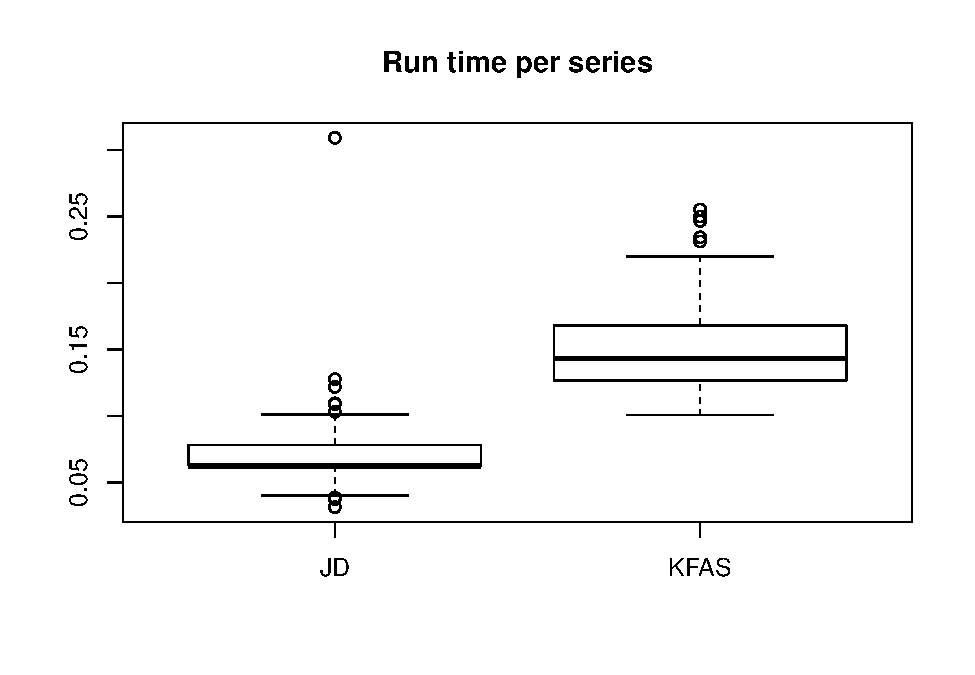
\includegraphics{simulation_test_files/figure-latex/simulate_sae-2.pdf}
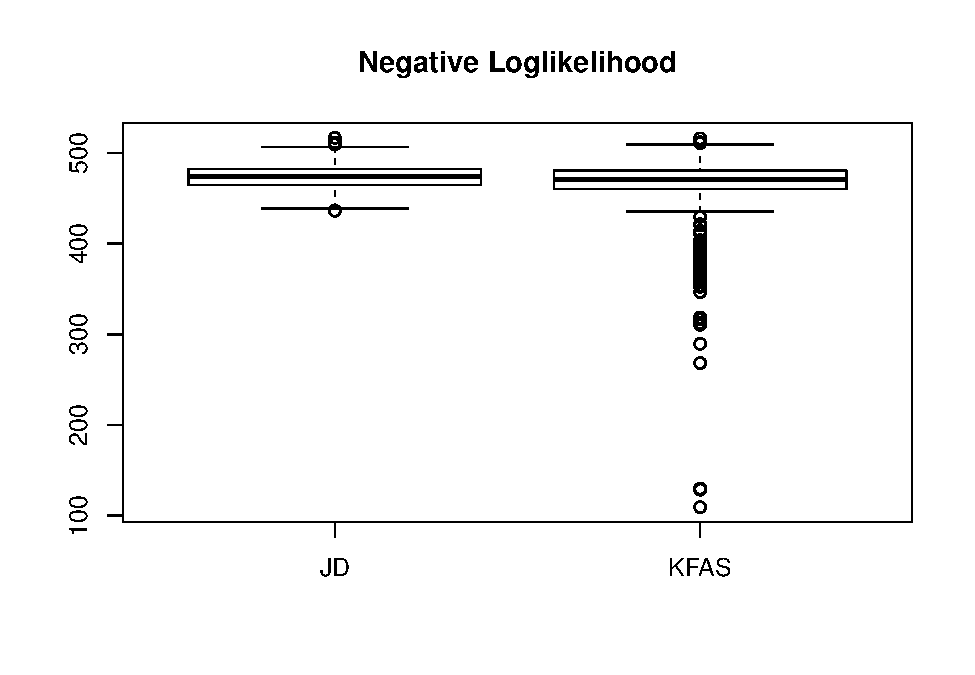
\includegraphics{simulation_test_files/figure-latex/simulate_sae-3.pdf}
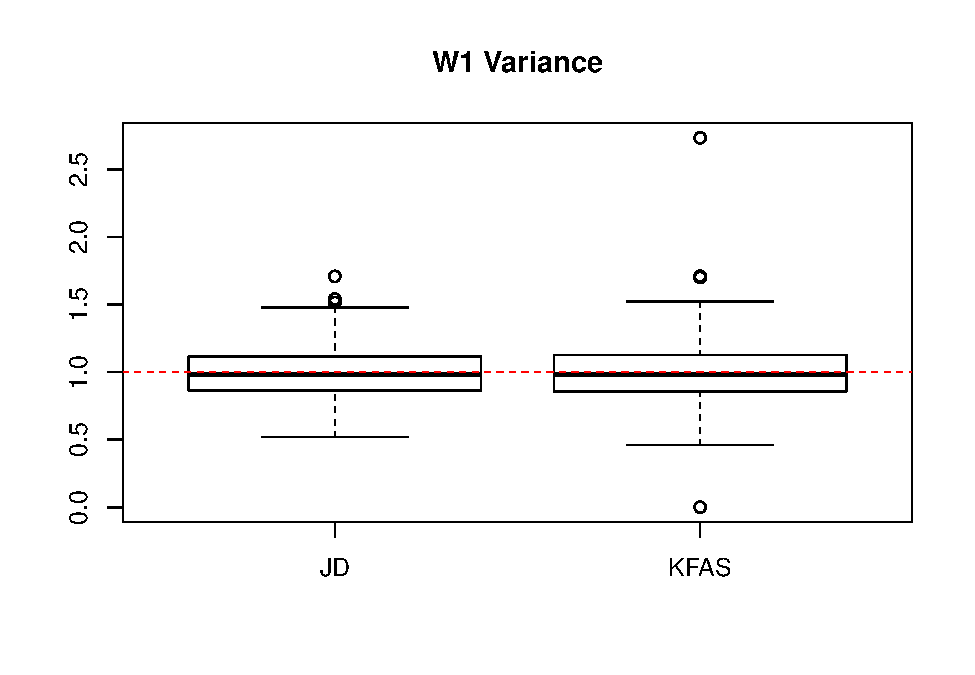
\includegraphics{simulation_test_files/figure-latex/simulate_sae-4.pdf}
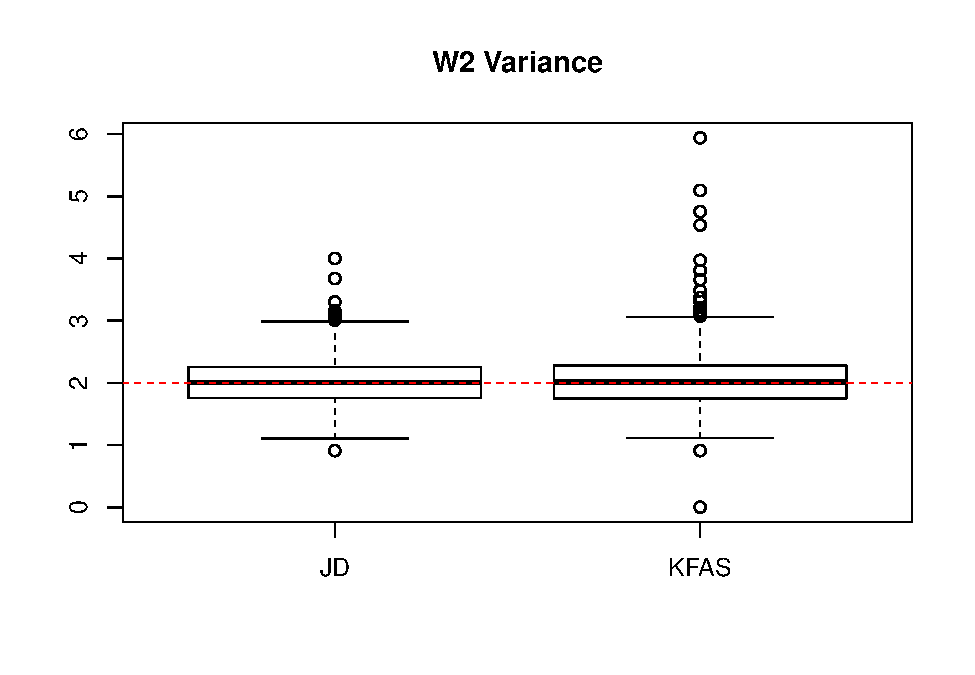
\includegraphics{simulation_test_files/figure-latex/simulate_sae-5.pdf}
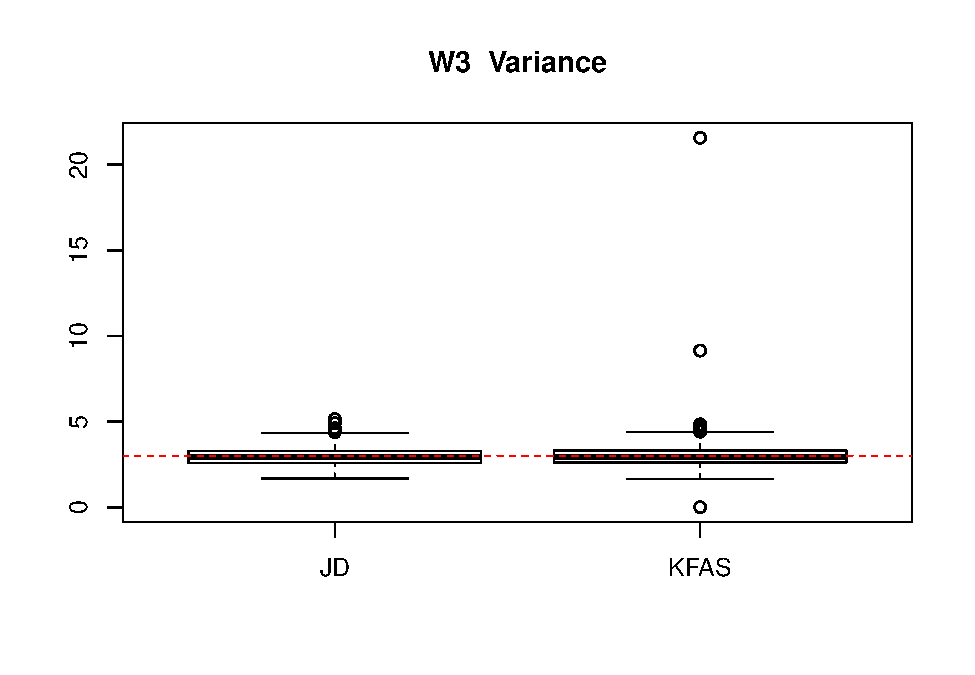
\includegraphics{simulation_test_files/figure-latex/simulate_sae-6.pdf}
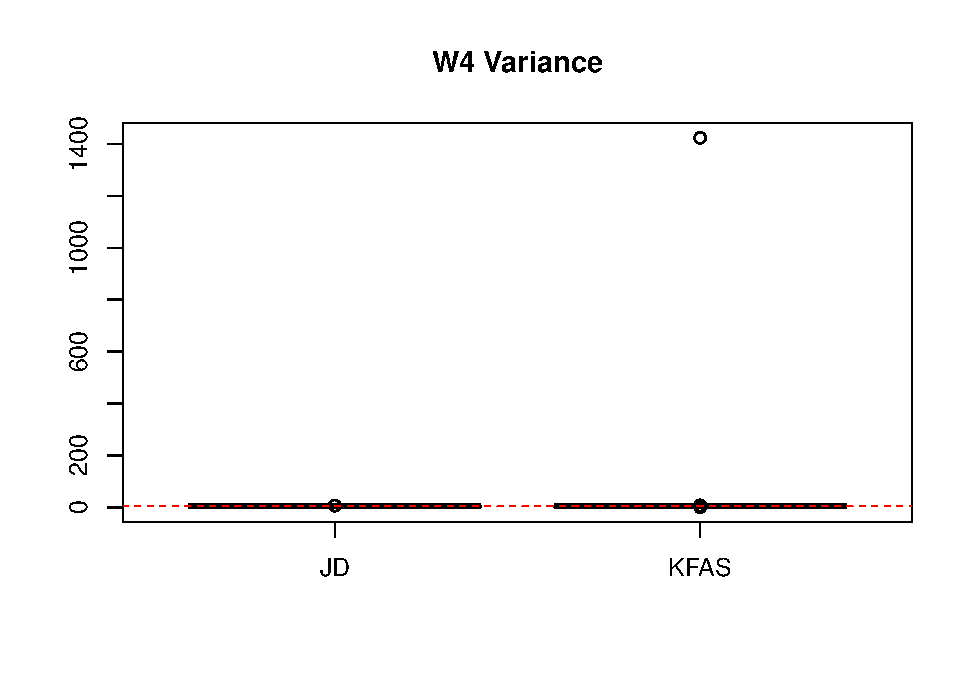
\includegraphics{simulation_test_files/figure-latex/simulate_sae-7.pdf}
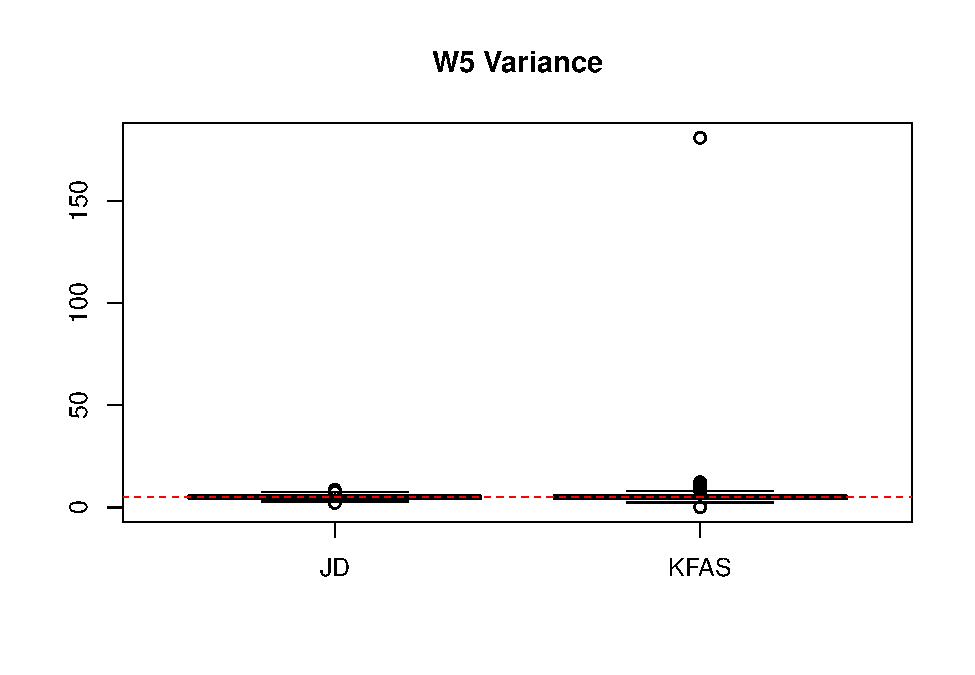
\includegraphics{simulation_test_files/figure-latex/simulate_sae-8.pdf}

\section{Simulation of SAE with bias}\label{simulation-of-sae-with-bias}

\begin{Shaded}
\begin{Highlighting}[]
\KeywordTok{print}\NormalTok{(}\StringTok{"Not done yet"}\NormalTok{)}
\end{Highlighting}
\end{Shaded}

\begin{verbatim}
## [1] "Not done yet"
\end{verbatim}

\section{Simulation of full model}\label{simulation-of-full-model}

\begin{Shaded}
\begin{Highlighting}[]
\KeywordTok{print}\NormalTok{(}\StringTok{"Not done yet"}\NormalTok{)}
\end{Highlighting}
\end{Shaded}

\begin{verbatim}
## [1] "Not done yet"
\end{verbatim}

\section{Actual series}\label{actual-series}

\begin{Shaded}
\begin{Highlighting}[]
\KeywordTok{load}\NormalTok{(}\StringTok{"../Data/retail.rda"}\NormalTok{)}
\NormalTok{n<-}\KeywordTok{length}\NormalTok{(retail)}
\NormalTok{jd_estimate <-}\StringTok{ }\OtherTok{NULL}
\NormalTok{kfas_estimate <-}\StringTok{ }\OtherTok{NULL}
\ControlFlowTok{for}\NormalTok{(i }\ControlFlowTok{in} \DecValTok{1}\OperatorTok{:}\NormalTok{n)\{}
\NormalTok{  y<-}\KeywordTok{log}\NormalTok{(retail[[i]])}
\NormalTok{   jd_start <-}\StringTok{ }\KeywordTok{Sys.time}\NormalTok{()}
\NormalTok{   q <-}\StringTok{ }\KeywordTok{jd_bsm}\NormalTok{(y,}\DataTypeTok{nar=}\DecValTok{0}\NormalTok{)}
\NormalTok{   jd_end <-}\StringTok{ }\KeywordTok{Sys.time}\NormalTok{()}
\NormalTok{   jd_dur <-}\StringTok{ }\NormalTok{jd_end}\OperatorTok{-}\NormalTok{jd_start}
\NormalTok{   s <-}\StringTok{ }\KeywordTok{result}\NormalTok{(q, }\StringTok{"scalingfactor"}\NormalTok{) }
\NormalTok{   p<-}\KeywordTok{result}\NormalTok{(q, }\StringTok{"parameters"}\NormalTok{)}
\NormalTok{   jd_estimate <-}\StringTok{ }\KeywordTok{rbind}\NormalTok{(jd_estimate,}\KeywordTok{as.numeric}\NormalTok{(}\KeywordTok{c}\NormalTok{(jd_dur,}\KeywordTok{result}\NormalTok{(q,}\StringTok{"loglikelihood"}\NormalTok{),s}\OperatorTok{*}\NormalTok{p[}\KeywordTok{c}\NormalTok{(}\DecValTok{1}\OperatorTok{:}\DecValTok{3}\NormalTok{)],s}\OperatorTok{*}\NormalTok{p[}\KeywordTok{length}\NormalTok{(p)]}\OperatorTok{*}\NormalTok{p[}\KeywordTok{length}\NormalTok{(p)])))}
\NormalTok{   kfas_start <-}\StringTok{ }\KeywordTok{Sys.time}\NormalTok{()}
\NormalTok{   r <-}\StringTok{ }\KeywordTok{kfas_bsm}\NormalTok{(y,init_val)}
\NormalTok{   kfas_end <-}\StringTok{ }\KeywordTok{Sys.time}\NormalTok{()}
\NormalTok{   kfas_dur <-}\StringTok{ }\NormalTok{kfas_end}\OperatorTok{-}\NormalTok{kfas_start}
\NormalTok{   kfas_estimate <-}\StringTok{ }\KeywordTok{rbind}\NormalTok{(kfas_estimate, }\KeywordTok{c}\NormalTok{(kfas_dur,}\OperatorTok{-}\NormalTok{r}\OperatorTok{$}\NormalTok{hyper_est}\OperatorTok{$}\NormalTok{optim.out}\OperatorTok{$}\NormalTok{value,}\KeywordTok{diag}\NormalTok{(r}\OperatorTok{$}\NormalTok{out}\OperatorTok{$}\NormalTok{model}\OperatorTok{$}\NormalTok{Q[,,}\DecValTok{1}\NormalTok{]),r}\OperatorTok{$}\NormalTok{out}\OperatorTok{$}\NormalTok{model}\OperatorTok{$}\NormalTok{H[,,}\DecValTok{1}\NormalTok{]))}
\NormalTok{\}}
\NormalTok{sim_end <-}\StringTok{ }\KeywordTok{Sys.time}\NormalTok{()}
\NormalTok{sim_dur <-}\StringTok{ }\NormalTok{sim_end}\OperatorTok{-}\NormalTok{sim_start}

\KeywordTok{print}\NormalTok{(}\KeywordTok{paste}\NormalTok{(}\StringTok{"Number of simulations ="}\NormalTok{,n))}
\end{Highlighting}
\end{Shaded}

\begin{verbatim}
## [1] "Number of simulations = 62"
\end{verbatim}

\begin{Shaded}
\begin{Highlighting}[]
\KeywordTok{print}\NormalTok{(}\KeywordTok{paste}\NormalTok{(}\StringTok{"JD+ average execution time ="}\NormalTok{,}\KeywordTok{sum}\NormalTok{(jd_estimate[}\DecValTok{1}\OperatorTok{:}\NormalTok{n,}\DecValTok{1}\NormalTok{])}\OperatorTok{/}\NormalTok{(n}\OperatorTok{-}\DecValTok{1}\NormalTok{)))}
\end{Highlighting}
\end{Shaded}

\begin{verbatim}
## [1] "JD+ average execution time = 0.0657891132792488"
\end{verbatim}

\begin{Shaded}
\begin{Highlighting}[]
\KeywordTok{print}\NormalTok{(}\KeywordTok{paste}\NormalTok{(}\StringTok{"KFAS average execution time ="}\NormalTok{,}\KeywordTok{sum}\NormalTok{(kfas_estimate[}\DecValTok{1}\OperatorTok{:}\NormalTok{n,}\DecValTok{1}\NormalTok{])}\OperatorTok{/}\NormalTok{(n}\OperatorTok{-}\DecValTok{1}\NormalTok{)))}
\end{Highlighting}
\end{Shaded}

\begin{verbatim}
## [1] "KFAS average execution time = 0.42526352210123"
\end{verbatim}

\begin{Shaded}
\begin{Highlighting}[]
\KeywordTok{print}\NormalTok{(}\StringTok{"JD+ likelihood - KFAS likelihood"}\NormalTok{)}
\end{Highlighting}
\end{Shaded}

\begin{verbatim}
## [1] "JD+ likelihood - KFAS likelihood"
\end{verbatim}

\begin{Shaded}
\begin{Highlighting}[]
\NormalTok{del<-jd_estimate[,}\DecValTok{2}\NormalTok{]}\OperatorTok{-}\NormalTok{kfas_estimate[,}\DecValTok{2}\NormalTok{]}
\KeywordTok{print}\NormalTok{(}\KeywordTok{summary}\NormalTok{(del))}
\end{Highlighting}
\end{Shaded}

\begin{verbatim}
##      Min.   1st Qu.    Median      Mean   3rd Qu.      Max. 
## -0.000004  0.000000  0.000217  1.002483  0.004891 18.587375
\end{verbatim}

\begin{Shaded}
\begin{Highlighting}[]
\KeywordTok{plot}\NormalTok{(del)}
\end{Highlighting}
\end{Shaded}

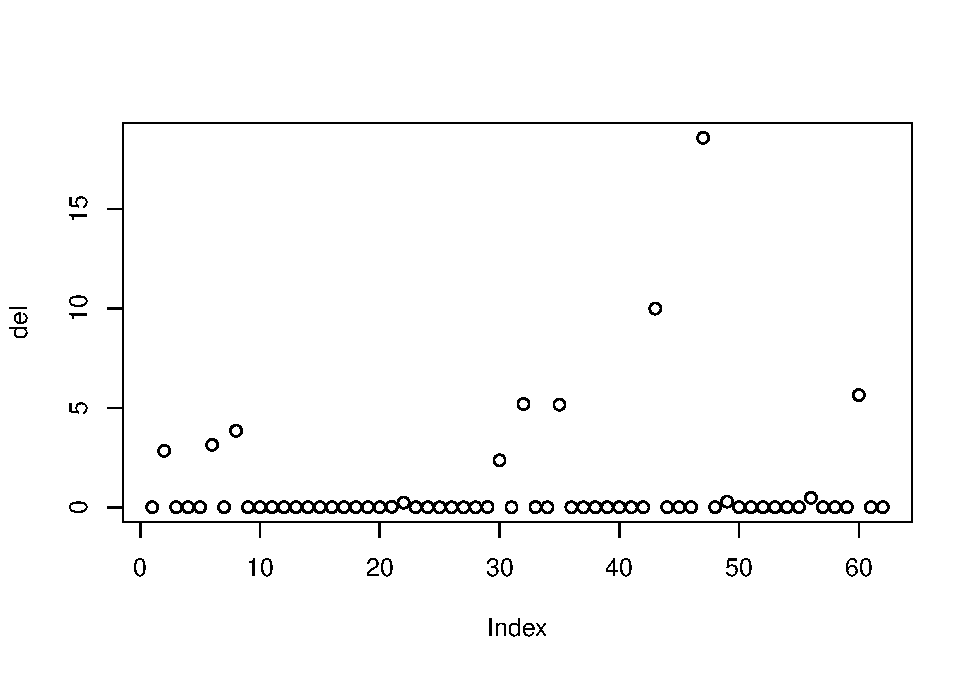
\includegraphics{simulation_test_files/figure-latex/unnamed-chunk-1-1.pdf}


\end{document}
